\section{Architecture globale du système}

Afin de répondre aux exigences de la transmission vidéo basse latence pour le pilotage 
FPV\index{FPV}, l'architecture du système a été pensée de manière modulaire. La chaîne de transmission 
a été segmentée en trois entités fonctionnelles et matérielles distinctes :

\begin{enumerate}
    \item \textbf{Le module d'acquisition et d'émission embarqué (TX) :} Destiné à être monté sur le 
    drone, il est chargé de la capture vidéo brute, de sa compression, et de son émission 
    radio sur la bande Sub-1 GHz.
    \item \textbf{Le pont réseau de réception au sol (routeur RX) :} Il agit comme une passerelle réseau 
    transparente. Son unique rôle est de réceptionner les ondes radio HaLow et de les convertir en trames 
    Ethernet physiques, sans effectuer de traitement logiciel.
    \item \textbf{La station de décodage et d'affichage :} Connectée au pont réseau via un câble Ethernet, 
    cette entité est exclusivement dédiée au traitement logiciel du flux vidéo entrant pour l'afficher 
    sur l'écran du pilote avec le délai le plus court possible.
\end{enumerate}

Cette segmentation offre un double avantage : elle permet de décharger les microcontrôleurs 
Wi-Fi des lourdes tâches d'encodage/décodage vidéo, et elle a rendu possible le profilage de 
chaque sous-système séparément tout au long de la phase de développement. Voici l'ensemble des plateformes matérielles ayant été évaluées.

% NOTE ÉTUDIANT : Schéma mis à jour intégrant la Debix en TX et le PC fixe 165Hz en RX
\begin{figure}[htbp]
    \centering
    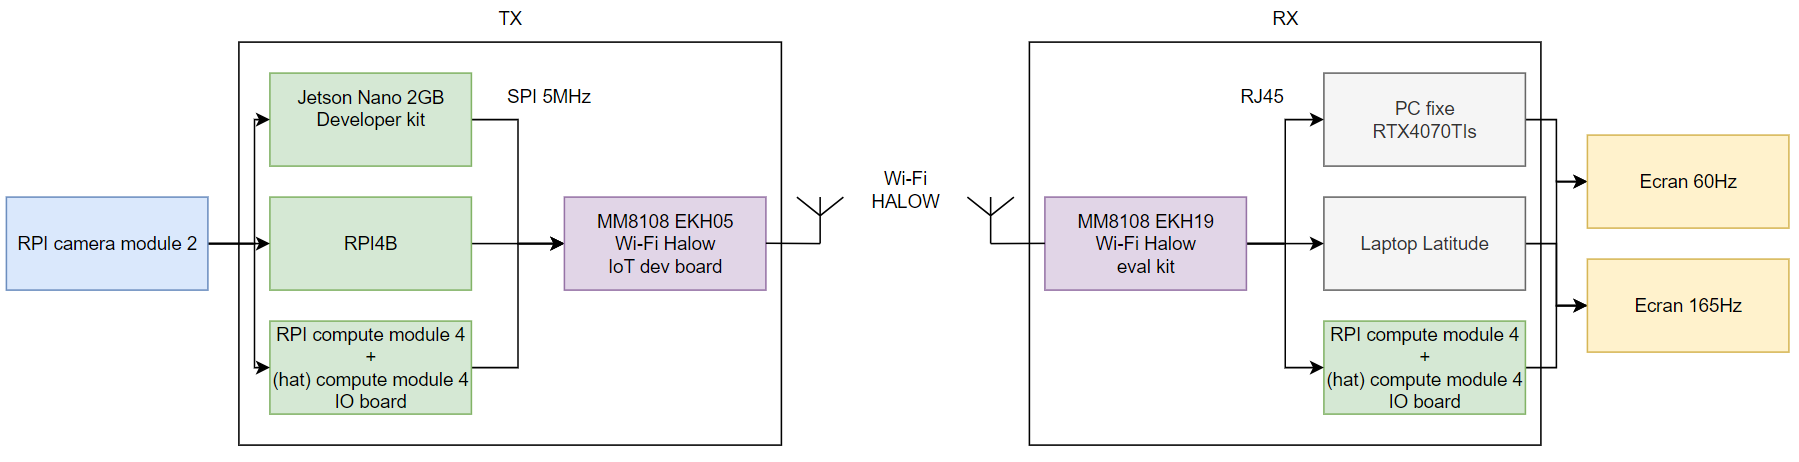
\includegraphics[width=1\textwidth]{imgs/complet_schematic.png}
    \caption{Architecture globale du système de transmission vidéo}
    \label{fig:arch_globale}
\end{figure}

\subsection{Le module d'acquisition et d'émission embarqué (TX)}
L'émetteur embarqué constitue le point de départ de la chaîne d'acquisition. Le choix du module de traitement 
vidéo et d'encodage a fait l'objet d'une sélection itérative parmi plusieurs ordinateurs monocartes :
\begin{itemize}
    \item Une \textbf{Nvidia Jetson Nano 2GB}\index{Jetson Nano} : Évaluée lors des premières phases d'expérimentation 
    pour valider la chaîne de transmission avec un encodeur matériel dédié (NVENC). Cette plateforme s'est 
    avérée logiciellement moins optimale pour notre application spécifique que l'écosystème Raspberry Pi. Elle a donc 
    été écartée suite à cette première phase de validation.
    \item L'écosystème \textbf{Raspberry Pi 4}\index{Raspberry Pi} (regroupant la \textit{Compute Module 4} et la 
    \textit{4B} classique en une seule architecture de référence) : Sélectionné comme la solution matérielle finale 
    pour l'émission. L'accès direct et hautement optimisé au processeur d'image (ISP) via l'outil natif \texttt{rpicam-vid} 
    s'est révélé nettement plus efficace en termes de latence brute que toutes les autres solutions testées.
    \item Une \textbf{Debix Model A}\index{Debix} : Évaluée brièvement pour ses capacités théoriques. Elle a rapidement 
    été écartée car l'exploitation de son accélération matérielle nécessitait l'utilisation de longs pipelines GStreamer 
    qui introduisaient plus de latence logicielle que l'implémentation directe et rationalisée de \texttt{rpicam-vid} 
    sur la Raspberry Pi.
\end{itemize}

Indépendamment de l'ordinateur monocarte retenu pour la compression, les trames segmentées sont transmises 
via un bus SPI\index{SPI} cadencé à 8 MHz vers un microcontrôleur \textbf{STM32U5}\index{STM32}. Ce MCU agit comme un 
pont matériel déterministe. Il encapsule les données vidéo entrantes dans des paquets UDP à l'aide de la pile 
réseau LwIP\index{LwIP}, avant de les expédier au module radio \textbf{Morse Micro MM8108 (EKH05)}\index{Wi-Fi HaLow!MM8108} 
pour la transmission RF sur la bande Sub-1 GHz.

\subsection{Le pont réseau de réception au sol (routeur RX)}
La réception des ondes HaLow est assurée par un routeur \textbf{GL.iNet MT3000} équipé d'une carte 
d'évaluation \textbf{EKH19}\index{EKH19}. Ce routeur, fonctionnant sous le système d'exploitation 
OpenWrt\index{OpenWrt}, est configuré pour agir comme un simple pont logiciel (\textit{Bridge}) transparent. 
Il réceptionne les trames 802.11ah sur son interface sans-fil et les injecte directement sur son interface 
Ethernet physique, limitant au maximum le temps de transit et le traitement par la pile TCP/IP interne du CPU.

\subsection{La station de décodage et d'affichage}
La station au sol est le dernier maillon de la chaîne, responsable du décodage et de l'affichage. Deux 
environnements ont été employés pour observer l'impact des couches d'abstraction d'affichage :
\begin{itemize}
    \item \textbf{La station cible (Raspberry Pi 4 / CM4) :} Utilisée lors du prototypage pour évaluer 
    des pipelines d'affichage KMS (\textit{Kernel Mode Setting}) afin de s'affranchir de l'overhead de l'OS. 
    \item \textbf{La station de décodage haute performance (PC fixe, GPU NVIDIA RTX 4070 Ti) :} Bien que l'architecture 
    cible finale d'un tel système soit embarquée, cette plateforme de diagnostic a été retenue pour l'établissement 
    de nos mesures de performance finales. Ce choix est principalement dicté par la nécessité d'utiliser un écran 
    haute fréquence, en l'occurrence \textbf{165 Hz}. Cette caractéristique est indispensable pour éliminer le goulot d'étranglement 
    temporel lié au taux de rafraîchissement d'un affichage standard (60 Hz), permettant de mesurer la latence glass-to-glass au 
    plus proche de sa valeur réelle.
\end{itemize}

\subsection{Architecture finale retenue pour le système}
Suite aux phases d'évaluations itératives, l'architecture optimale et stabilisée retenue pour l'évaluation finale du système s'articule autour des composants matériels et logiciels suivants :
\begin{itemize}
    \item \textbf{Côté Émetteur (TX) :} Une caméra Raspberry Pi V2 reliée à une Raspberry Pi 4B (CPU isolé sur le cœur 3, overclocké à 2.0 GHz). Le flux vidéo est capturé et compressé à la volée au format MJPEG à l'aide de l'outil \texttt{rpicam-vid} (320x240, 60 FPS, Qualité 8). Les trames sont découpées et poussées sur le bus SPI cadencé à 8 MHz par notre passerelle en C (\texttt{gateway\_spi.c}) vers la carte de transmission STM32U5/MM8108 (EKH05).
    \item \textbf{Liaison Radio :} Modulation fixe forcée en MCS 1 (8 MHz de largeur de bande) utilisant le protocole UDP Unicast avec un marquage agressif de la Qualité de Service MAC (WMM/EDCA file "Voice") et la désactivation totale du mode d'économie d'énergie (PSM).
    \item \textbf{Côté Récepteur (RX) :} La carte de réception EKH19 reliée en bus interne au routeur OpenWrt GL.iNet MT3000, configurée en simple pont Ethernet transparent vers notre PC fixe de diagnostic (décodage GStreamer logiciel sans synchronisation et affichage direct sur l'écran haute vitesse 165 Hz).
\end{itemize}
\begin{figure}[htbp]
    \centering
    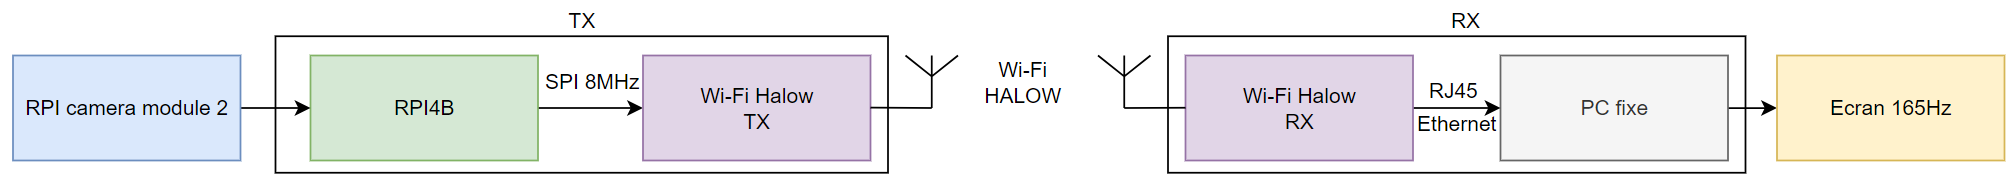
\includegraphics[width=1\textwidth]{imgs/final_schematic.png}
    \caption{Architecture retenue}
    \label{fig:final_schematic}
\end{figure}


\subsection{Flux logique du système}
L'articulation des composants et le cheminement des données à travers les quatre grands maillons du système 
sont modélisés par la figure \ref{fig:complet_schematic_nb}.

\begin{figure}[htbp]
    \centering
    
\includegraphics[width=1\textwidth]{imgs/complet_schematic_nb.png}
    \caption{Flux logique du système : (1) Lien réseau Sub-1 GHz, (2) Capture vidéo, (3) Plateformes de traitement, (4) Interfaçage SPI.}
    \label{fig:complet_schematic_nb}
\end{figure}